\chapter{Conclusions}
\label{ch:conclusions}

\textbf{This chapter is now complete - but wasn't in the first three chapter draft submission!}

In conclusion, this project assesses Rust as suitable for performant and production implementations of High-Performance Computing codebases, answering the titular question. This conclusion is as a result of three factors.

Firstly, \Cref{ch:translation} shows that it is possible to translate non-trivial existing codebases representative of High-Performance Computing workloads from C++ into Rust, including leveraging both shared and distributed memory parallelism through the \texttt{rayon} and \texttt{mpi} crates. It further shows that these translations provide significant benefits to developer productivity. These include reduced effort spent debugging as a result of memory and concurrency safety guarantees and the rich type system, along with quantitative models of productivity using the \texttt{scc} tool suggesting around a $0.61 \times$ total cost to complete develop the codebase with both shared and distributed memory parallelism in Rust.

Secondly, \Cref{ch:performance} shows that the performance of Rust translations of non-trivial C++ codebases closely approaches their reference implementations, with at worst around a $1.5 \times$ slowdown incurred across parallelism strategies. In addition to this, the Rust translations exhibit similar strong and weak scaling properties to the original C++ implementations, demonstrating its capability to scale to the extent required for High-Performance Computing workloads. These performance measurements concur with existing literature, such as Moran and Bull's ``Emerging Technologies: Rust in HPC'' \cite{moranEmergingTechnologiesRust2023}.

These first two factors can be interpreted together by plotting a graph comparing the empirical performance and estimated productivity of C++ and Rust implementations of the HPCCG mini-app, as shown in Figure \ref{fig:conclusions_performance_productivity}. This figure visualises the fact that C++ offers fair performance gains over Rust, but development of Rust programs is likely to improve development productivity.

\begin{figure}[H]
    \centering
    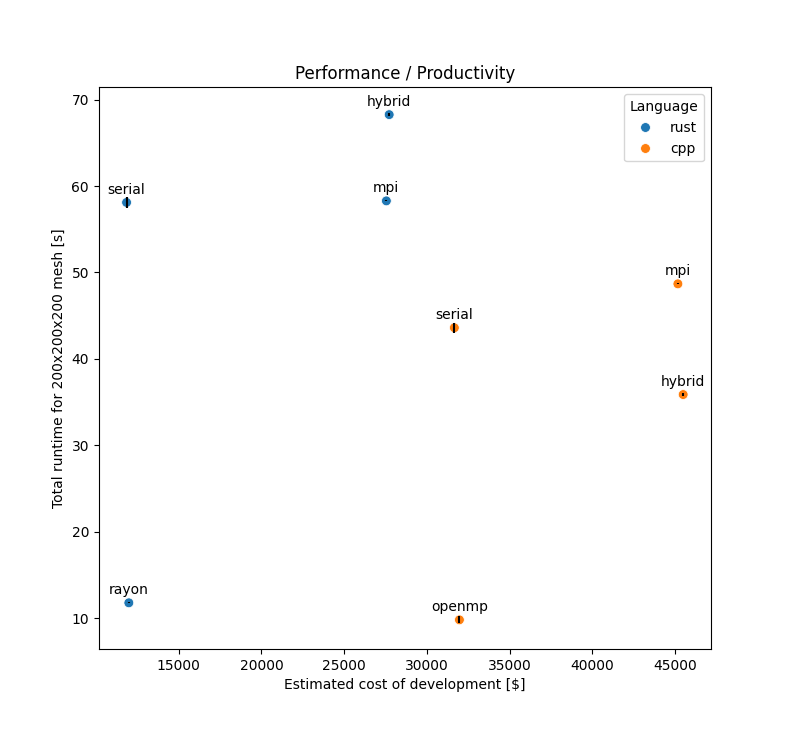
\includegraphics[width=\textwidth]{images/7_conclusions/performance_productivity.png}
    \caption{A comparison of performance and productivity between the C++ and Rust languages.}
    \label{fig:conclusions_performance_productivity}
\end{figure}

% scc . --exclude-file Cargo.lock --exclude-dir target
% scc . --exclude-file .gitignore YAML* dump_matlab*
% name,performance (200^3 in s),scc cost($)
% serial,58.1+/-0.6,11844
% rayon(32),11.77+/-0.04,11980
% mpi,58.28+/-0.05,27553
% hybrid,68.26+/-0.19,27723
% Do the header comments mess this up?
% serial,43.6+/-0.6,31665
% openmp(32),9.8+/-0.4,31970
% mpi,48.68+/-0.05,45180
% hybrid,35.87+/-0.17,45500

The final factor which impacts the conclusion is that Rust's performance and productivity are likely to improve faster than C++. This is because it is a relatively young language, whose package ecosystem and optimising compilers are still under active development and hence yet to reach maturity.

These factors taken in combination demonstrate Rust's suitability for High-Performance Computing applications, as despite its performance not matching C++, it provides commensurate benefits in developer productivity such as its compiler guarantees of memory and thread safety, which might make it preferable for real-world applications bounded by budget.


% This project was a success, as it achieved all of its ``Must have'' and ``Should have'' objectives, shown in Appendix \ref{sec:project-requirements}. These include translating, equivalence checking, and undertaking a performance analysis of a High-Performance Computing mini-app across serial, shared memory, and distributed memory parallelism approaches. In addition to this, two ``Could have'' objectives relating to the equivalence checking were dropped, which allowed time for the development of tooling for reproducibly running and aggregating performance experiments. This tool facilitated deep performance analysis of the HPCCG translation, but also stands on its own as a helpful utility for engineers working in High-Performance Computing, as validated by the industry review.


\section{Reflection}
\label{sec:reflection}

% It can be a useful exercise for you (and a point of consolidation for the reader) to put together a brief summary of what you have achieved. This is not a compulsory section, but a self-assessment is welcome. A suggested format for this is to include a short section entitled 'Author's Assessment of the Project' consisting of brief (up to 100 words) answers to each of the following questions.
%     What is the (technical) contribution of this project?
%     Why should this contribution be considered relevant and important for the subject of your degree?
%     How can others make use of the work in this project?
%     Why should this project be considered an achievement?
%     What are the limitations of this project?

On reflection, I am immensely proud of the work I have completed in the course of this project. Coming in to the project, I did not have a good way to estimate how long translation tasks, so generously scheduled time in my project specification to undertake these tasks. It transpired that I was able to complete the translation of the serial and parallel implementations faster than expected, which allowed me to focus on the stretch goals of the project. The initially planned stretch goal was extending the translation effort to include an assessment of the Rust bindings to MPI. This presented an interesting technical challenge of using complex Rust structures within an API which does not exactly map the C++ implementation of the MPI specification.

In addition to this, empowered by incredibly helpful conversations with my supervisor, I also chose to extend the project by building tooling to facilitate performance measurements on High-Performance Computing resources using Slurm. I found this very fulfilling, as I personally enjoy building tooling, and was able to apply knowledge about what makes real-world tools effective that I learnt on my year in industry. In my opinion, this is one of the stand-out aspects of this project, as it not only was it incredibly helpful during my performance analysis, but can also be used as an open source software product going forward.


\section{Future work}
\label{sec:future-work}

Whilst HPCCG is around an order of magnitude longer than any of the Rust codebases examined in existing literature, it is one of the shortest mini-apps in the Mantevo suite. In addition to this, other mini-apps are more influential in within this space, with HPCCG just being the first to introduce the idea. As a result of this, one avenue for future work is translating and analysing a longer, more influential mini-app, for example MiniMD \cite{osti_1231191} or HPCG \cite{dongarra2015hpcg}.

Secondly, equivalence checking is a very broad and complex field. As such, future work could easily be derived from this section. For example, a framework implementing the proof-of-concept for the \texttt{autocxx} approach to test-driven development could be developed, for example by using Rust macros for ergonomic multiplexing between C++ and Rust function calls. In addition to this, comparison of generated LLVM IR for equivalence checking was dropped as out of scope for this project, but could still yield fruitful research.

% In addition to this, publicising and maintaining open source tools requires a lot of effort from developers. To maximise the impact of the HPC MultiBench, a final possible avenue of future work is making it easily accessible, including publishing it on to the Python Package Repository, and responding to bug and feature requests raised on GitHub.

Finally, I am aiming to submit a paper derived from this project to the P3HPC (Performance, Portability and Productivity in High-Performance Computing) 2024 workshop, based on the novel contributions discussed in \Cref{ch:introduction}.


\section{Open source work}
\label{sec:open-source-work}

The open source community is critical in publishing and maintaining much of the infrastructure the modern world runs on
% with and estimated xyz devices running the Linux kernel \cite{}
. In the course of this project, the author developed a number of open source contributions.

Due to the departmental regulations on open source contributions, the vast majority of open source contributions developed during this project are embargoed in private repositories, which will then be made public after the assessment phase of the project has completed. However, there are some exceptions to this policy, which were made with supervisor approval.

\section{Contributions already released}
\label{sec:open-source-already-released}

% TODO: Re-order to be coolest first.
Firstly, during the initial mini-app identification phase of the project, I noticed that some of the links on the UK-MAC website were broken. As a result of this, I raised a GitHub issue for this (\url{https://github.com/UK-MAC/uk-mac.github.com/issues/1}), and then made a pull request to fix these links (\url{https://github.com/UK-MAC/uk-mac.github.com/pull/2}). This pull request has since been merged, and the website now works correctly.

Secondly, when developing the novel equivalence checking approach leveraging foreign-function interfaces in Rust with \texttt{autocxx}, I needed to invoke functions using array parameters. There was an open issue (\url{https://github.com/google/autocxx/issues/989}) on the project stating that some support for arrays had recently been added, but that this functionality was untested. To resolve this, I pull requested in integration tests for this functionality (\url{https://github.com/google/autocxx/issues/989}), which confirms its correctness and prevent regression in future.

% TODO: Move to appendices
% , shown in Figure \ref{fig:autocxx_pr}. 
% \begin{figure}[H]
%     \centering
%     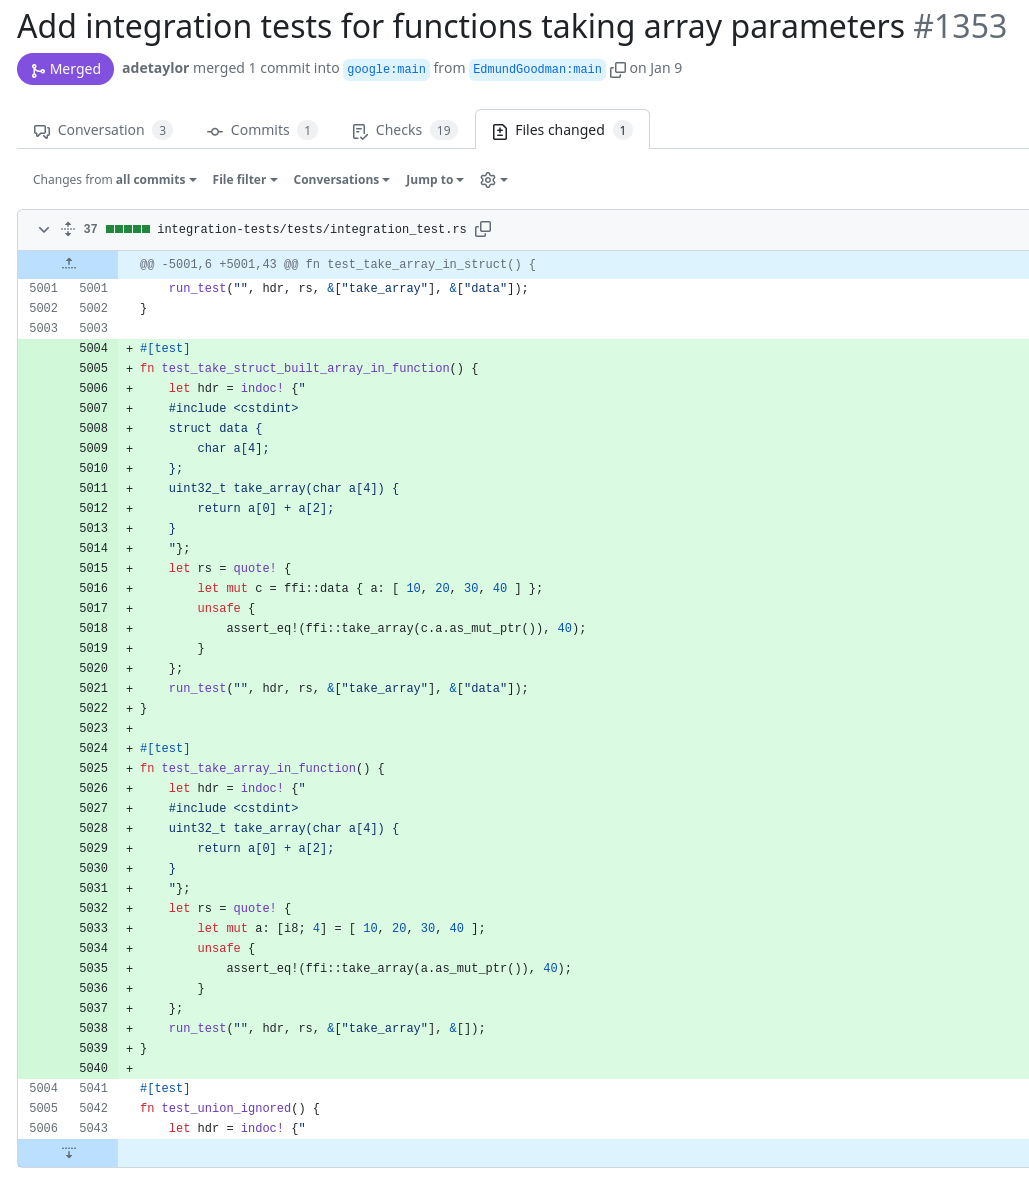
\includegraphics[width=\textwidth]{images/7_conclusions/autocxx_pr.png}
%     \caption{A screenshot of the pull request adding integration tests for array support made into \texttt{autocxx}.}
%     \label{fig:autocxx_pr}
% \end{figure}

This pull request has since been merged into the main branch in this repository, and as such will be included in the next release of the \texttt{autocxx} tool. Since this functionality is very common in High-Performance Applications, this confirmation of support unblocks applying this technique in future work

Finally, I made a pull request into the HPCCG repository to add Doxygen-style docstrings to the mini-app, based on the understanding that I gained during the translation process \url{https://github.com/Mantevo/HPCCG/pull/5}. However, since this project was last actively developed seven years ago, this pull request has not been reviewed nor merged.

\section{Contributions to be released}
\label{sec:open-source-to-be-released}

In addition to these contributions, the following contributions have already been written and will be made once the project has been assessed:

\begin{enumerate}
    \item Make public the HPC MultiBench tool, and publish it on PyPI so it can be installed using the \texttt{pip} package manager
    \item Make public the Rust translation of the HPCCG mini-app
    \item Make public the run results generated using the HPC MultiBench tool for the Rust translation of HPCCG and the replication trial of Moran and Bull's paper \cite{moranEmergingTechnologiesRust2023}
    \item Pull request modernisation of the build system for the HPCCG mini-app to use CMake
    \item Pull request unit tests using the Catch2 framework written the for HPCCG mini-app
    \item Pull request a link to Kokkos version of the HPCCG mini-app into \url{https://github.com/kokkos/kokkos-miniapps}, a repository containing a list of mini-apps with Kokkos translations
\end{enumerate}

Finally, I intend to write then make the following contributions once the project has been assessed:

\begin{enumerate}
    \item Pull request documentation for using arrays as function arguments in \texttt{autocxx}, following up on the pull request discussed in the previous section \url{https://github.com/google/autocxx/pull/1353#issuecomment-1961615591}
    \item Pull request documentation including and annotating integration tests as examples for the \texttt{mpi} crate, following up on issue \url{https://github.com/rsmpi/rsmpi/issues/174#issuecomment-1961638459}.
\end{enumerate}
